% THIS IS SIGPROC-SP.TEX - VERSION 3.1
% WORKS WITH V3.2SP OF ACM_PROC_ARTICLE-SP.CLS
% APRIL 2009

\documentclass{acm_proc_article-sp}

\usepackage{todonotes}
\usepackage{algorithm}
\usepackage{url}
\usepackage[noend]{algpseudocode}
\usepackage{mdframed}
\usepackage{amsmath}

\newtheorem{defn}{\textbf{Definition}}
\newtheorem{thm}{\textbf{Theorem}}
\newtheorem{cor}{\textbf{Corollary}}
\newtheorem{lemma}{\textbf{Lemma}}

\begin{document}

\title{AND\=aNA-v2: Application-Layer Support for \\ Low-Latency Bidirectional Anonymous Traffic in NDN}

\numberofauthors{3} 
\author{
% 1st. author
\alignauthor
Christopher A. Wood\titlenote{NSF GRFP blurb.}\\
       \affaddr{University of California Irvine}\\
       \affaddr{Irvine, CA, USA}\\
       \email{woodc1@uci.edu}
% 2nd. author
\alignauthor
Gene Tsudik\\
       \affaddr{University of California Irvine}\\
       \affaddr{Irvine, CA, USA}\\
       \email{gts@ics.uci.edu}
% 3rd. author
\alignauthor 
Ersin Uzun\\
       \affaddr{Computer Science Laboratory}\\
       \affaddr{PARC}\\
       \affaddr{Palo Alto, CA, USA}\\
       \email{Ersin.Uzun@parm.com}
}
\date{\today}

\maketitle
\begin{abstract}
TODO
\end{abstract}

% A category with the (minimum) three required fields
\category{H.4}{TODO}{TODO}
%A category including the fourth, optional field follows...
\category{D.2.8}{TODO}{TODO}[TODO]

\terms{TODO}

\keywords{TODO} % NOT required for Proceedings

\section{Introduction} \label{sec:introduction}
Usage of the Internet has undergone a tremendous transformation since its inception in the 1970s. Content distribution, as opposed to point-to-point communication, has become the leading type of traffic traversing today's valuable network resources; Netflix, for example, accounted for nearly 30\% of all downstream traffic in 2012 \cite{Netflix}. The number and popularity of such information-centric services are only expected to increase in the future with the growing presence of data-intensive consumer applications and devices (e.g., media streaming applications and mobile devices), leading to added pressure on network resources and a subsequent increase in network congestion and wasted bandwidth. 

Named-data networking (NDN) \cite{ndn-techreport} is an emerging network architecture capable of supporting information-centric traffic. Two primary characteristics of the NDN architecture are that content names, rather than hosts or locations, are addressible and routable through the network, and all generated content corresponding to some name must be signed by its original producer. The latter property decouples content confidentiality, integrity, and authenticity from content and the manner in which it is delivered to consumers (e.g., instead of using secure tunnels akin to SSH/TLS, content can be encrypted before sent to a consumer). These fundamental design decisions enable content to be cached in network-layer resources throughout the network, thus promoting reduced network congestion and wasted bandwidth when popular content is requested. 

The NDN design builds content security support \emph{into the architecture} and promotes content access via producer-specified forms of encryption. Similar to the IP-based counterpart, consumer and producer anonymity, however, are not readily supported by this design. While there are no longer source or destination addresses associated with traffic, there are a variety of other sources of information via which consumers can be deanonymized, including: interest and content names, network router cache contents, and digital signature contents. An intelligent adversary may use any of these information sources when launching client deanonymization attacks. 

{\sf AND\=aNA}, an anonymous named-data networking application, pioneered support for anonymous content retrieval and distribution with regards to consumers and producers, respectively \cite{andana}. Inspired by Tor \cite{Tor}, {\sf AND\=aNA} uses onion-encryption to wrap requests for content that are iteratively decrypted and forwarded by participating anonymizing routers, and also to wrap content as it flows from the producer to the consumer. Unlike Tor, however, {\sf AND\=aNA} was a proof-of-concept application-layer anonymizing layer for NDN that targeted unidirectional traffic \emph{without} real-time requirements. Support for high-throughput, low-latency, bidirectional traffic, such as traffic generated from voice communication, video chat, and media streaming applications. In addition to this severe performance impediment, the ``optimized'' session-based variant of {\sf AND\=aNA} sacrificed interest and content linkability (an anonymity issue) for only slightly improved efficiency. 

Consequently, in this work we present a new and substantially improved design for an NDN anonymizng application, henceforth referred to as {\sf AND\=aNAv2}, that addresses the many performance and anonymity pitfalls of the original design. We discuss the design and implementation of {\sf AND\=aNAv2} as built upon CCNx \cite{ccnx}, the open-source relative of NDN. We also present performance results from testing our application implementation in numerous test environments with different types of traffic. Our results show that our modified design leads to  substantial performance gains without sacrificing consumer or producer privacy, thus making {\sf AND\=aNAv2} a promising application to support a diverse set of application content and use cases in future information-centric networks.

\section{Preliminaries} \label{sec:preliminaries}
In this section we give a more detailed overview of the properties of the NDN architecture relevant to the issue of anonymous communication. We then also delve into the design of AND\=aNA (henceforth referred to as AND\=aNA-v1), to identify the major security flaws and engineering shortcomings that are remedied in AND\=aNA-v2. 

\subsection{NDN Overview}
Named-data networking (NDN) is one of several proposed information-centric network designs under active research and development as the future Internet architecture. Its defining characteristic is that it decouples the location of data from its original publisher. All requested content is cached in network-layer routers between consumers who request data and publishers, or other routers, satisfying such data. In essence, network caches and addressable content, rather than addressable hosts or interfaces, enable this new architecture to reduce network congestion and latency by keeping content closer to its intended recipients. 

Content is requested through the issuance of an \emph{interest}, or a meaningful URI with a one-to-one correspondence with content provided by the network. The components of an interest are arbitrary strings and can therefore be used to store any type of data, including human readable names or binary data encoded as URI-friendly strings. Upon receiving an interest, a router looks for a match in its \emph{content store} (CS), which is the cache that stores content already requested from other consumers. Matching is done using exact-match based on content names, i.e., a complete interest name match in the CS will cause the associated content to be forwarded downstream on the same router interface upon which the interest arrived. Interests that do not completely match any content name in the CS are stored in a \emph{pending interest table} (PIT) together with the corresponding interface upon which the interest arrived and is subsequently forwarded to the appropriate upstream router based on contents in a \emph{forward interest base} (FIB) table. Multiple interests matching the same name are collapsed into a single PIT entry to prevent redundant interests being sent upstream. Once a content matching a PIT entry is received by a router, the content is cached (unless the interest has explicitly marked the content to not be stored) and sent to all downstream interfaces associated with the PIT entry. Finally, upon completion, the PIT entry is cleared.

Content-centric traffic also has strong security implications. Firstly, it means that content security is tied to the data itself, not the channel through which it flows between consumers and the network. All sensitive content must therefore be protected with a suitable form of encryption to ensure confidentiality. Content integrity is guaranteed by digital signatures; all content producers are required to sign content before responding to incoming interests. Due to performance impediments, signature verification is not required by network routers; naturally, consumer applications are expected to verify content signatures. Issues regarding signature verification and key management are discussed more at length in \cite{}.Secondly, a lack of source and destination addresses improves user privacy. However, as we will discuss in the following section, this lack of information is insufficient with regards to consumer privacy. 

\subsection{Notions of Anonymity}
\todo[inline]{I think a section dedicated to anonymity and relevant definitions is warranted here, oui?}

\subsection{AND\=aNA-v1 Design Highlights}
Section \ref{sec:design} provides a detailed description of the design of {\sf AND\=aNA-v2}, which is inspired by Tor and its predecessor, {\sf AND\=aNA-v1}. To motivate our changes we first describe the {\sf AND\=aNA-v1} design in sufficient detail. As previously mentioned, {\sf AND\=aNA-v1} achieves anonymous communication using mix behavior analogous to Tor; Interests for content are wrapped in layers of encryption, where each encrypted layer has sufficient information necessary to forward the interest to the correct anonymizing router. Note that unlike Tor, persistent circuits with long-term TCP connections are not established with {\sf AND\=aNA-v1}. Rather, ephemeral circuits are created as an interest is decrypted and forwarded upstream towards the consumer. State information in each anonymizing router is only maintained in the symmetric (session-based) variant of {\sf AND\=aNA-v1}. Once a piece of content is retrieved corresponding to an interest, each anonymizing router wraps it with a layer of encrypting using a public or symmetric key specific in the corresponding interest, and is subsequently sent back downstream. In this way, circuits only exist for the duration of a single interest-content retrieval. This behavior is illustrated in Figure \ref{fig:andanav1_design}.

\begin{figure}
\begin{center}
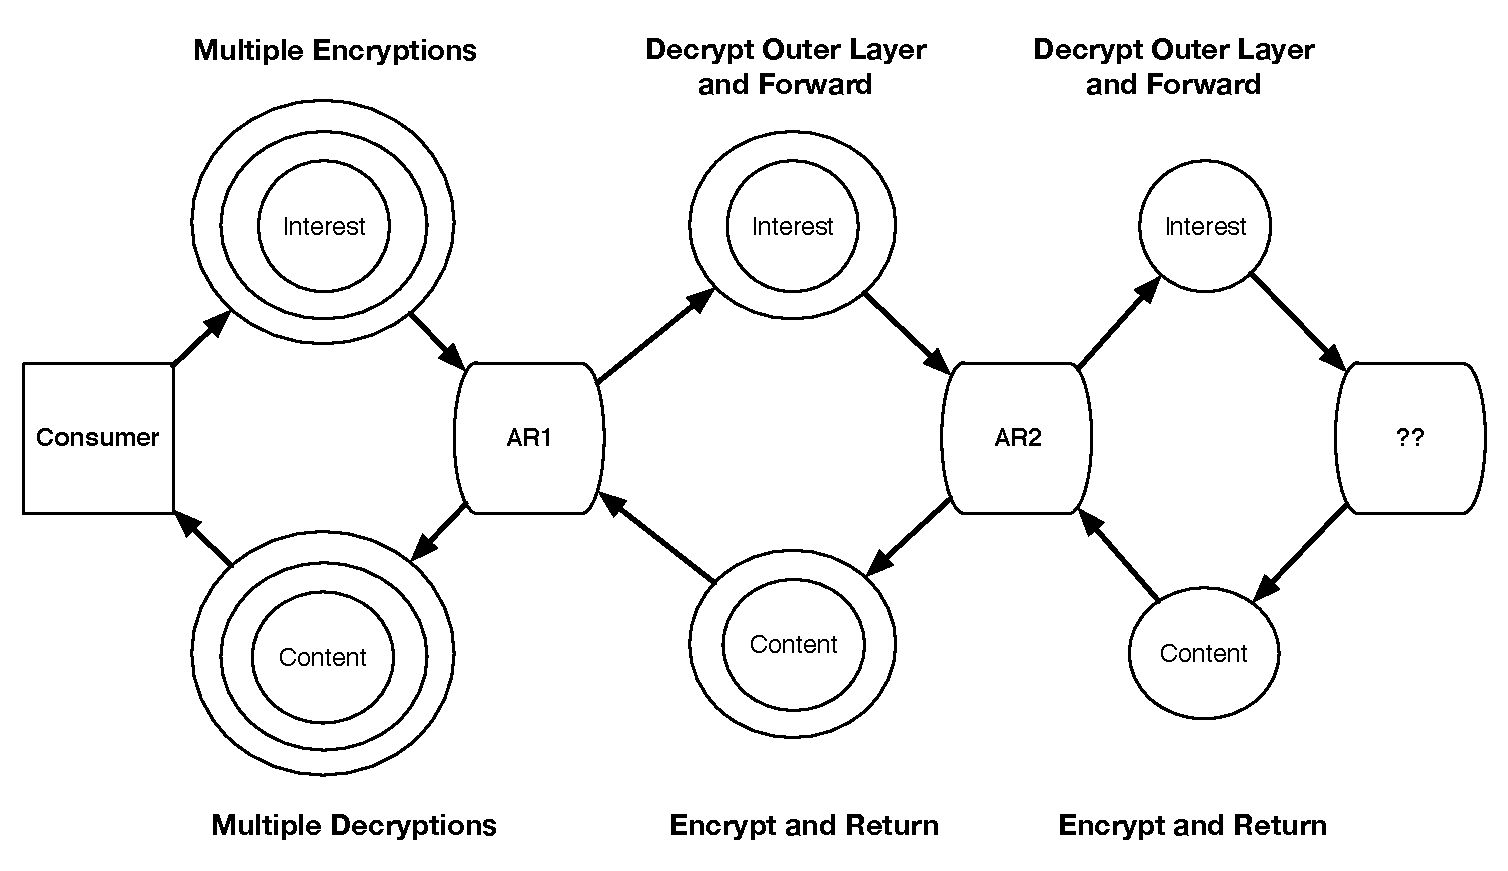
\includegraphics[scale=0.34]{./images/andana_v1_design.pdf}
\label{fig:andanav1_design}
\caption{Interest and content onion encryption and decryption in the original {\sf AND\=aNA-v1} design.}
\end{center}
\end{figure}

In the symmetric variant of {\sf AND\=aNA-v1}, state information consisting of a unique session identifier and symmetric key used for interest and content decryption and encryption, respectively, is established and persisted in each anonymizing router using a standard three-way handshake protocol. While the use of symmetric encryption removes the computational burden of asymmetric content encryption, the reference design required that the session identifier be sent in the clear for every interest, allowing an adversary to link packets and content together and render the consumer susceptible to a deanonymization attack (see the following section for more details). Furthermore, not only is the initial state establishment protocol composed of interests that are distinct from regular encrypted interests, the handshake procedure wastes consumer bandwidth and time when used for short-term anonymous traffic. 

\todo[inline]{We can probably go farther here - has the point been driven home?}

\subsection{Pitfalls and Shortcomings}
The primary motivation for a new design of {\sf AND\=aNA} is to attain the same anonymity and privacy guarantees as {\sf AND\=aNA} with \emph{better} performance. The original design targeted a single use case in which performance, especially in the bidirectional setting, was not a primary concern. Indeed, there was both an asymmetric and symmetric (session-based) variant of {\sf AND\=aNA}, and while the latter enjoyed better speedups over the former by using symmetric encryption it suffered the fatal flaw of not ensuring packet unlinkability. It is generally the case that unlinkability is merely sufficient for anonymity, rather than also being a necessary condition for anonymity. However, in the case of {\sf AND\=aNA}, packet linkability can lead to consumer and producer linkability, which immediately violates anonymity. For example, it is not difficult to hypothesize an adversary that eavesdrops on incoming and outgoing interests for a particular anonymous router, and who by doing so is able to determine that the incoming and outgoing session IDs are linked. In fact, a modified type of this kind of adversary was explicitly studied in the context of Tor by Murdoch and Danezis in \cite{tor-traffic-analysis}. In their work, the goal of the adversary in their ``linkability attack'' was to determine whether two separate data streams being served by two corrupted servers were initiated by the same consumer, and we suspect that such analysis could be augmented to work for {\sf AND\=aNA}. Specifically, repeating a packet linkability attack at each anonymous router in a circuit may therefore eventually lead to linkability between the producer and consumer. 

The use of application and environment contextual information has also been formally studied in \cite{attacking-unlinkability}, in which side channel and environment information (e.g., the deterministic behavior of an anonymous router always forwarding a packet upstead after unwrapping an interest received from some downstream router) is used to quantify the \emph{degree of unlinkability}. Furthermore, we remark that regardless of how such linkability information is acquired, it has been shown that it can lead to reduce consumer and producer anonymity beyond what is possible with general traffic analysis \cite{linkability-attacks}. 

As most of the literature focuses on mix-based anonymizing services akin to Tor, which inspired the original design of {\sf AND\=aNA}, it is clear that any form of linkability should be avoided in order to maintain consumer and producer anonymity. Therefore, one formal goal for {\sf AND\=aNA-v2} is to attain the same anonymity and privacy guarantees as the asymmetric variant of {\sf AND\=aNA}, which does not suffer from packet linkability issues, while supporting \emph{superior} performance in the low-latency, high-throughput, bidirectional traffic use case when compared to the symmetric variant of {\sf AND\=aNA}.

\section{AND Design} \label{sec:design}
In this section we describe the much improved design of {\sf AND}. Table \ref{tab:notation} introduces the relevant notation needed to understand the design in its entirety. 

\begin{table*}
\centering
\caption{Notation used in the presentation of this work.}
\label{tab:notation}
  \begin{tabular}{| r | l |} \hline
  $\mathsf{C}$ & Set of all consumers  \\
  $\mathsf{P}$ & Set of all producers  \\ 
  $\mathsf{R}$ & Set of all routers  \\
  $\mathsf{IF}$ & Set of all interfaces on all routers  \\
  $\mathsf{if}_i^r \in \mathsf{IF}$ & Interface $i$ of router $r$  \\
  $\kappa$ & The global security paramter (set to $256$ in practice) \\ 
  $(pk_i, sk_i)$ & Public/private key pair for router $r$  \\
  $\overline{\mathsf{int}}_{i}^{j}$ & Encrypted interest wrapped from router $i$ to router $j$ ($i \leq j$)  \\
  $\mathcal{A}$ & Adversary \\ 
  $u$ & Entity in the network (consumer or producer) \\
  $u \to_{\mathsf{int}} r$ & Entity $u$ sends interest to router $r$  \\ 
  $\mathsf{int} \to \mathsf{if}_i^r$ & Interest $\mathsf{int}$ is sent to interface $i$ of router $r$ \\
  $r \in \mathsf{R}$ & An anonymizing router (AR) \\ 
  $\mathcal{E}_{pk_i}(\cdot)$ & Public key encryption using $pk_i$ \\ 
  $\mathcal{D}_{pk_i}(\cdot)$ & Public key decryption using $pk_i$ \\ 
  $\mathsf{Encrypt}_{k_i}(\cdot)$ & Symmetric key encryption using key $k_i$ \\ 
  $\mathsf{Decrypt}_{k_i}(\cdot)$ & Symmetric key decrypt using key $k_i$ \\ 
  $\mathsf{ST}$ & AR session table used to store session ID and digest tuples \\
  $H$ & A collision resistant hash function on the domain $\{0,1\}^*$ to range $\{0,1\}^{\kappa}$ \\
  $F_k$ & A keyed pseudorandom function \\ \hline
  \end{tabular}
\end{table*}

\subsection{Circuit and Session Establishment}
At the heart of the {\sf AND} is the notion of anonymizing routers and connection-oriented circuits, similar in spirit to the inner workings of TOR \cite{Tor}. Anonymizing routers serve two purposes in {\sf AND}: (1) to decapsulate and forward encrypted interests, along with content encryption keys, generated by a consumer until the cleartext interest arrives at the producer, and (2) to encapsulate sensitive content using the previously acquired encryption keys and relay the encrypted content downstream. In this way, the consumer generates an interest wrapped by several layers of encryption and receives a piece of content wrapped in several layers of encryption that it can easily decrypt. It is also important to note that since each anonymizing router operates at the application layer, it effectively serves as the producer for each downstream router in the {\sf AND} circuit. Therefore, NDN policy dictates that such content \emph{must be signed}. Verification of content from upstream routers, however, is not mandatory. 

We also note that the current {\sf AND} design has support for two types of circuits: asymmetric and symmetric session-based. In the asymmetric variant, all encrypted interests are done using a CCA-secure PKI scheme and all content is encrypted using a CCA-secure symmetric key encryption scheme. Conversely, in the session-based variant, all encrypted interests are protected using a CCA-secure symmetric key encryption scheme, where the key is identified using a unique session identifier sent in the cleartext along with the encrypted interests. This worsens anonymity because it provides a way to link packets to a single session (as previously discussed).

Putting together all of the design aspects of the current version of {\sf AND}, we see that the following factors weigh in on the overall performance of the application: content encryption, content signature generation, and encrypted interest generation. In {\sf AND} we seek to minimize the degree to which these factors affect interest and content encapsulation and decapsulation by integrating support for anonymous router \emph{state}, which is encapsulated in sessions, into anonymous circuits. Sessions will exist for unidirectional traffic only, which therefore means that bidirection traffic, the ultimate focus of this work, will require two sessions to be established and maintained for the duration of the bidirectional application. This is done so that each party in the application need not use the same set of anonymous routers for communication. Not only does this free each consumer to select a random subset of anonymous routers $r_1,r_2,\dots,r_n$ from the set of total anonymous routers $\mathsf{R}$, but it may also help improve QoS guarantees by distributing the load of encapsulation and decapsulation among multiple nodes. Furthermore, sessions enable the establishment of long-term secrets that can be used to improve the efficiency of certain cryptographic operations, such as content encryption, signature generation, and signature verification. 

With the end of goal of supporting highly efficient and anonymous bidirectional traffic, the goals of the circuit and session establishment using a list of $n$ anonymous routers $r_1,\dots,r_n$ are as follows:
\begin{enumerate}
\item Establish unique session IDs $\mathsf{session}_{i}$ and session IVs $\mathsf{SIV}_i$
\item Establish content encryption keys $E_{k_i}$ and initial counter values $\mathsf{EIV}_i$
\item Establish pairwise MAC keys $M_{k_i}$ between adjacent routers and the consumer used to tag and verify content
\end{enumerate}

The purpose of each of these session entities will become clear from the circuit initialization and usage procedures. After establishment, the circuit from the consumer $C$ to the producer $P$ should be similar to that shown in Figure \ref{fig:circuit}. We now describe the general protocol for establishing this type of session-based circuit from a consumer $C$ to a producer $P$ given $n$ anonymous routers. Recall that, in order to support bidirectional communication, $P$ would have to establish a similar circuit to $C$ with $m$ routers, where $m$ need not equal $n$. 

{\sf AND} supports state initialization that is separate in time from circuit usage (i.e., using a handshake routine to initialize the state) as well as one that initializes session state upon issuance of the first wrapped consumer interest. In what follows we describe the handshake variant of session establishment. Online session establishment, used to remove the seemingly unnecessary handshake phase altogether, is discussed in Section \ref{sec:piggyback}.

\begin{algorithm*}[ht!]
  \caption{Circuit and Session Establishment Protocol}
  \begin{algorithmic}[1]
    \Require{Anonymous routers $r_1,r_2,\dots,r_n$ ($n \geq 1$) with public keys $pk_1,pk_2,\dots,pk_n$.}

% \Function{{\sf ServerRetrieveMACKey}}{$\mathsf{int}$} %// Server-side at router $i$
%   \State $(M_{k}, \mathsf{session}_i, x) := \mathcal{D}_{sk_i}(\mathsf{int}[-1])$ %// Recover MAC key and randomness $x$
%   \If{$\mathsf{session}_i$ not in state}
%     \State \Return $\mathsf{Error}$
%   \Else
%     \State Persist $M_k$ as $M_{k_{i+1}}$ (the upstream MAC key) with session $\mathsf{session}_i$
%     \State $x^* := \mathsf{MAC}_{M_{k}}(x)$
%     \State $\mathsf{resp} := x^*$
%     \State \Return $\mathsf{resp}$
%   \EndIf

%   % \State $(E_{k_n}, M_{k_n}, \mathsf{EIV}_n, \mathsf{session}_n, \mathsf{SIV}_n) \gets \overline{\mathcal{D}_{k}}(T)$
%   % \State \Return $(E_{k_n}, M_{k_n}, c_n, \mathsf{session}_n, \mathsf{IV}_n)$
% \EndFunction

\medskip

\Function{{\sf ServerEstablishSession}}{$\mathsf{int}$} %// Server-side at router $i$
  % \State $k \gets \mathcal{D}_{sk_i}(\mathsf{int}[-1])$ %// Recover session encryption key
  % \State $E_{k_i} \gets \{0,1\}^{\kappa}$ %// Encryption key
  % \State $M_{k_i} \gets \{0,1\}^{\kappa}$ %// MAC key
  % \State $\mathsf{EIV}_i \gets \{0,1\}^{\kappa}$ %    // counter IV
  % \State $x \gets \{0,1\}^{\kappa}$
  % \State $\mathsf{SIV}_i \gets \{0,1\}^{\kappa}$ %// session IV
  % \State $\mathsf{session}_i := H(x)$ %// session ID
  % \State $\mathsf{SIndex}_i := H(\mathsf{session}_i + \mathsf{SIV}_i)$
  \State $(k, E_{k_i}, M_{k_i}, M_{k_{i+1}}, \mathsf{EIV}_i, \mathsf{SIV}_i, \mathsf{session}_i, \mathsf{SIndex}_i) := \mathcal{D}_{sk_i}(\mathsf{int})$
  \State Persist $(\mathsf{session}_i, E_{k_i}, M_{k_i}, M_{k_{i+1}}, \mathsf{EIV}_i, \mathsf{SIV}_i)$ to state, and store $(\mathsf{SIndex}_i, \mathsf{session}_i, \mathsf{SIV}_i)$ in the session table $\mathsf{ST}_i$
  \State $\mathsf{resp} \gets \mathsf{Encrypt}_{k}(\mathsf{session}_i, E_{k_i}, M_{k_i}, \mathsf{EIV}_i, \mathsf{SIV}_i)$
  \State \Return $\mathsf{resp}$
  
  % \State $T' := \mathcal{D}_{sk}(T)$ // Secret key $sk$ corresponding to the receiving router $r$
  % \If {$|T'| = 4$}
  %   \State Persist $(\mathsf{session}, E_{k}, c, M_{k})$ to state
  % \Else
  %   \State Persist $(\mathsf{session}, E_{k}, c, M_{k}, M_{k_{+1}})$ to state
  % \EndIf
\EndFunction

\medskip

% \Function{{\sf ClientSendMACKey}}{$r_i$, $\mathsf{session}_i$, $M_{k}$} // Client-side
%   \State $x \gets \{0,1\}^{\kappa}$
%   \State $x' := \mathsf{MAC}_{M_{k}}(x)$
%   \State $T \gets \mathcal{E}_{pk_i}(M_{k}, \mathsf{session}_i, x)$
%   \State $\mathsf{int} := \mathsf{namespace}_i/\mathsf{SESSIONMAC}/T$
%   \State $\mathsf{resp} := \mathsf{ccnget}(\mathsf{int})$ // reach out to the AR
%   \State $x^* := \mathsf{resp}[-1]$
%   \If{$x' \not= x^*$}
%     \State \Return $\mathsf{Fail}$
%   \Else
%     \State \Return $\mathsf{Pass}$
%   \EndIf

%   % \State $(E_{k_n}, M_{k_n}, \mathsf{EIV}_n, \mathsf{session}_n, \mathsf{SIV}_n) \gets \overline{\mathcal{D}_{k}}(T)$
%   % \State \Return $(E_{k_n}, M_{k_n}, c_n, \mathsf{session}_n, \mathsf{IV}_n)$
% \EndFunction

\Function{{\sf ClientEstablishSession}}{$r_i$, $M_{k_{i+1}}$} %// Client-side
  % \State $k \gets \{0,1\}^{\kappa}$
  % \State $\overline{k} \gets \mathcal{E}_{pk_i}(k)$

  % \State $k \gets \mathcal{D}_{sk_i}(\mathsf{int}[-1])$ %// Recover session encryption key
  \State $E_{k_i} \gets \{0,1\}^{\kappa}$ %// Encryption key
  \State $M_{k_i} \gets \{0,1\}^{\kappa}$ %// MAC key
  \State $\mathsf{EIV}_i \gets \{0,1\}^{\kappa}$ %    // counter IV
  \State $x \gets \{0,1\}^{\kappa}$
  \State $\mathsf{SIV}_i \gets \{0,1\}^{\kappa}$ %// session IV
  \State $\mathsf{session}_i := H(x)$ %// session ID
  \State $\mathsf{SIndex}_i := H(\mathsf{session}_i + \mathsf{SIV}_i)$

  \State $\mathsf{int} := \mathsf{namespace}_i/\mathsf{CREATESESSION}/\mathcal{E}_{pk_i}(k, E_{k_i}, M_{k_i}, M_{k_{i+1}}, \mathsf{EIV}_i, \mathsf{SIV}_i, \mathsf{session}_i, \mathsf{SIndex}_i)$
  \State $\mathsf{resp} := \mathsf{ccnget}(\mathsf{int})$ // reach out to the AR
  % \State $(E_{k_n}, M_{k_n}, \mathsf{EIV}_n, \mathsf{session}_n, \mathsf{SIV}_n) \gets \mathsf{Decrypt}_{k}(\mathsf{resp})$
  \State \Return $(E_{k_i}, M_{k_i}, x_i, \mathsf{session}_i, \mathsf{IV}_i)$
\EndFunction

% \State $E_{k_i} \gets \{0,1\}^k$ for $k = 1,\dots,n$ // Encryption key
% \State $M_{k_i} \gets \{0,1\}^k$ for $k = 1,\dots,n$ // MAC key
% \State $c_i \gets \{0,1\}^k$ for $k = 1,\dots,n$     // counter IV
% \State $x \gets \{0,1\}^k$
% \State $\mathsf{session}_n := H(x)$
% \State $T' := (\mathsf{session}_n, E_{k_n}, c_n, M_{k_n})$
% \State $T_n := \mathcal{E}_{pk_n}(T')$

\medskip

\Function{{\sf EstablishCircuit}}{$r_1,\dots,r_n$} %// Main procedure
\State $(E_{k_n}, M_{k_n}, c_n, \mathsf{session}_n, \mathsf{IV}_n) := \mathsf{ClientEstablishSession}(r_n)$
\For{$i = n - 1$ \textbf{ downto } $1$}
  \If{$i = n-1$}
    \State $(E_{k_i}, M_{k_i}, \mathsf{EIV}_i, \mathsf{session}_i, \mathsf{SIV}_i) := \mathsf{ClientEstablishSession}(r_i, \perp)$
  \Else
    \State $(E_{k_i}, M_{k_i}, \mathsf{EIV}_i, \mathsf{session}_i, \mathsf{SIV}_i) := \mathsf{ClientEstablishSession}(r_i, M_{k_{i+1}})$
  \EndIf
  % \If{$\mathsf{ClientSendMACKey}(r_i, \mathsf{session}_i, M_{k_{i+1}}) = \mathsf{Fail}$}
    % \State \Return $\mathsf{Fail}$
  % \EndIf
  % \State $\mathsf{session}_{i} := H(\mathsf{session}_n \bigoplus_{j=i}^{n} E_{k_j})$
  % \State $T' := (\mathsf{session}_i, E_{k_i}, c_i, M_{k_i}, M_{k_{i+1}})$
  % \State $T_n := \mathcal{E}_{pk_i}(T_i)$
  % \State $\mathsf{EstablishSession}(T_i)$
\EndFor
\EndFunction

  \end{algorithmic}
\end{algorithm*}

Notice that by this procedure, no two routers will share the same session identifier (with non-negligible probability) even though they partake in the same circuit. This is because they generate session identifiers independent and uniformly at random from $\{0,1\}^{\kappa}$. 

% \begin{figure*}[ht!]
% \begin{center}
% 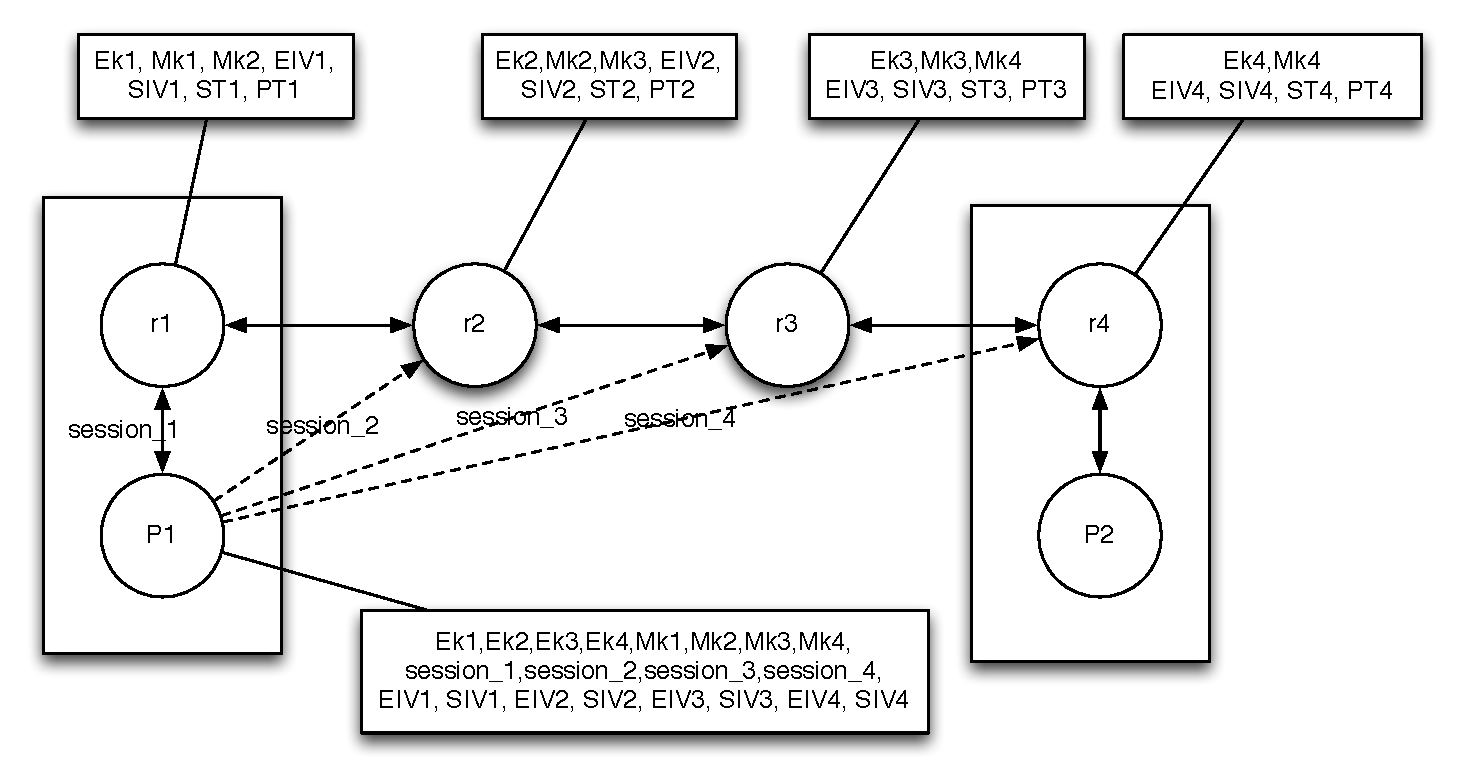
\includegraphics[scale=0.5]{./images/circuit.pdf}
% \end{center}
% \caption{Sample session-based circuit between a consumer $C$ and producer $P$ with ARs $r_1,r_2,r_3,r_4$, where the end routers on the path are run on the same node as $C$ and $P$.}
% \label{fig:circuit}
% \end{figure*}

\subsection{AND Circuit Usage}

We note that anonymous routers must be chosen in a \emph{mutually excluse} manner, meaning that they do not change share the same name prefix or are from the same organization (see Figure \ref{fig:pool}). This requirement is needed for ensuring anonymity. After a circuit and the corresponding sessions have been created between the consumer and each anonymous router, usage of the circuit proceeds as per the original {\sf AND} design. Specifically, there are three main operations that need to be defined: encrypted interest generation, AR interest forwarding, and AR content handling. In what we follows we present the details of each of these procedures as needed for {\sf AND}. We begin with the encrypted interest generation procedure (shown in Algorithm \ref{alg:enc_int_gen}) in which a consumer $C$ particpating in a particular \emph{application} session with a producer $P$ wraps an interest for the session to be sent into the anonymizing circuit. A wrapped (encrypted) interest from $r_i$ to $r_j$ ($i \leq j$) is denoted as $\overline{\mathsf{int}}_i^j$, meaning that the original plaintext interests $\mathsf{int}$ cannot be retrieve unless encrypted by each router $r_i,r_{i+1},\dots,r_j$, in that order. Thus, the original wrapped interest is denoted as $\overline{\mathsf{int}}_1^n$.

\begin{figure*}[ht!]
\begin{center}
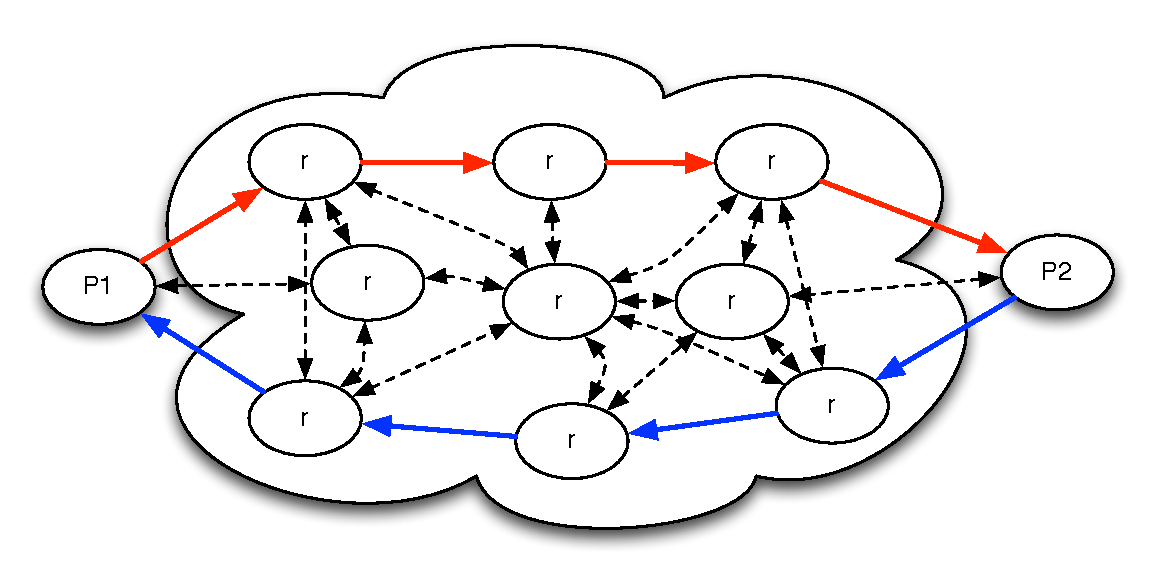
\includegraphics[scale=0.5]{./images/pool.pdf}
\end{center}
\caption{A sample bidirectional circuit configuration in which two parties communicate using mutually exclusive ARs in both directions. Note that it is not required for each circuit to be the same length, nor is it required that the intersection of the routers for each direction of the circuit to be empty (i.e., routers may \emph{unknowingly} support sessions traversing in both directions).}
\label{fig:pool}
\end{figure*}

\begin{algorithm}[ht!]
  \caption{Encrypted Interest Generation}
  \begin{algorithmic}[1]
    \Require{Interest $\mathsf{int}$, circuit length $n$, AR pool $\mathcal{R}$}
    \Ensure{Encrypted interest $\overline{\mathsf{int}}_{1}^{n}$}
\State $\overline{\mathsf{int}} = \mathsf{int}$
\For{$i = n$ \textbf{ downto } $1$}
  \State $\mathsf{SIndex}_i := H(\mathsf{session}_i + \mathsf{SIV}_i)$
  \State $\mathsf{SIV}_i = \mathsf{SIV}_i + 1$ (mod $2^{\kappa}$)
  \State $\overline{\mathsf{int}}_i^n = R_i / \mathsf{SIndex}_i / \mathsf{Encrypt}_{E_{k_i}}(\overline{\mathsf{int}}, \mathsf{timestamp})$
\EndFor
\State \Return $\overline{\mathsf{int}}_1^n$
\end{algorithmic}
\label{alg:enc_int_gen}
\end{algorithm}

\begin{algorithm*}[ht!]
  \caption{AR Encrypted Interest Forwarding}
  \begin{algorithmic}[1]
    \Require{$\overline{\mathsf{int}}_i^j$}
    \Ensure{$(\overline{\mathsf{int}}_{i+1}^j, \mathsf{session}_i)$ or discarded packet}
\If{$\mathsf{SIndex}_i \in \mathsf{ST}_i$}
  \State Let $(\mathsf{session}_i, E_{k_i}, M_{k_i}, \mathsf{EIV}_i, \mathsf{SIV}_i)$ be the session information associated with $\mathsf{SIndex}_i$
  \State $\mathsf{SIV}_i := \mathsf{SIV}_i + 1$ (mod $2^{\kappa}$)
  \State $\mathsf{SIndex}_i := H(\mathsf{session}_i + \mathsf{SIV}_i)$
  \State Update $(\mathsf{SIndex}_i, \mathsf{session}_i, \mathsf{SIV}_i)$ in the session table $\mathsf{ST}_i$
  \State $(\overline{\mathsf{int}}_{i+1}^{j}, timestamp) := \mathsf{Decrypt}_{E_{k_i}}(\overline{\mathsf{int}}_{i}^{j})$
  \If{decryption fails or $\mathsf{timestamp}$ is not current}
    \State Discard $\overline{\mathsf{int}}_{i}^{j}$
  \Else
    \State Persist tuple $T_i = (\overline{\mathsf{int}}_{i}^{j}, \overline{\mathsf{int}}_{i+1}^{j}, \mathsf{session}_i)$ to pending interest table $\mathsf{PT}_i$
    \State \Return $(\overline{\mathsf{int}}_{i+1}^{j}, \mathsf{session}_i)$
  \EndIf
\Else
  \State Discard $\overline{\mathsf{int}}_{i}^{j}$ %\Comment{Some form of interest flooding prevention should be employed here}
\EndIf
\end{algorithmic}
\label{alg:enc_int_forward}
\end{algorithm*}

\begin{algorithm}[ht!]
  \caption{AR Content Handling}
  \begin{algorithmic}[1]
    \Require{Content $\overline{data_{i+1}^j}$ in response to interest $\overline{\mathsf{int}}_{i+1}^{j}$}
    \Ensure{Encrypted data packet $data_{i}^j$}
\State Recover tuple $T_i = (\overline{\mathsf{int}}_{i}^{j}, \overline{\mathsf{int}}_{i+1}^{j}, \mathsf{session}_i)$ based on $data_{i+1}^j$
\State Parse $\overline{data_{i+1}^j}$ as a tuple $(data_{i+1}^j, \sigma_{i+1})$
\If{$\sigma_{i+1} = \epsilon$ and $M_{k_{i+1}} = \epsilon$} %\Comment{Last hop router - does not verify MAC}
  \State Pass
\ElsIf{$\sigma_{i+1} \not= \epsilon$ and $M_{k_{i+1}} \not= \epsilon$}
  \If{$\sigma_{i+1} = \mathsf{Verify}_{M_{k_{i+1}}}(data_{i+1}^j)$}
    \State Pass
  \Else
    \State \Return $\mathsf{Error}$ %\Comment{MAC verification did not pass}
  \EndIf
\Else %\Comment{There was either a tag or we don't have the upstream MAC key - either way, we error}
  \State \Return $\mathsf{Error}$
\EndIf

\State Remove signature and name from $data_{i+1}^j$    
\State Create new empty data packet $data_i^j$
\State Set name on $data_i^j$ as the name on $\overline{\mathsf{int}}_{i}^{j}$
\State $data_i^j := \mathsf{Encrypt}_{E_{k_i}}(data_i^j)$
\State $\sigma_i := \mathsf{MAC}(data_i^j)$
\State $\overline{data_{i}^j} = (data_i^j, \sigma_i)$
\State \Return $\overline{data_{i}^j}$

\end{algorithmic}
\label{alg:ar_content_handler}
\end{algorithm}

% \begin{figure*}[ht!]
% \begin{center}
% 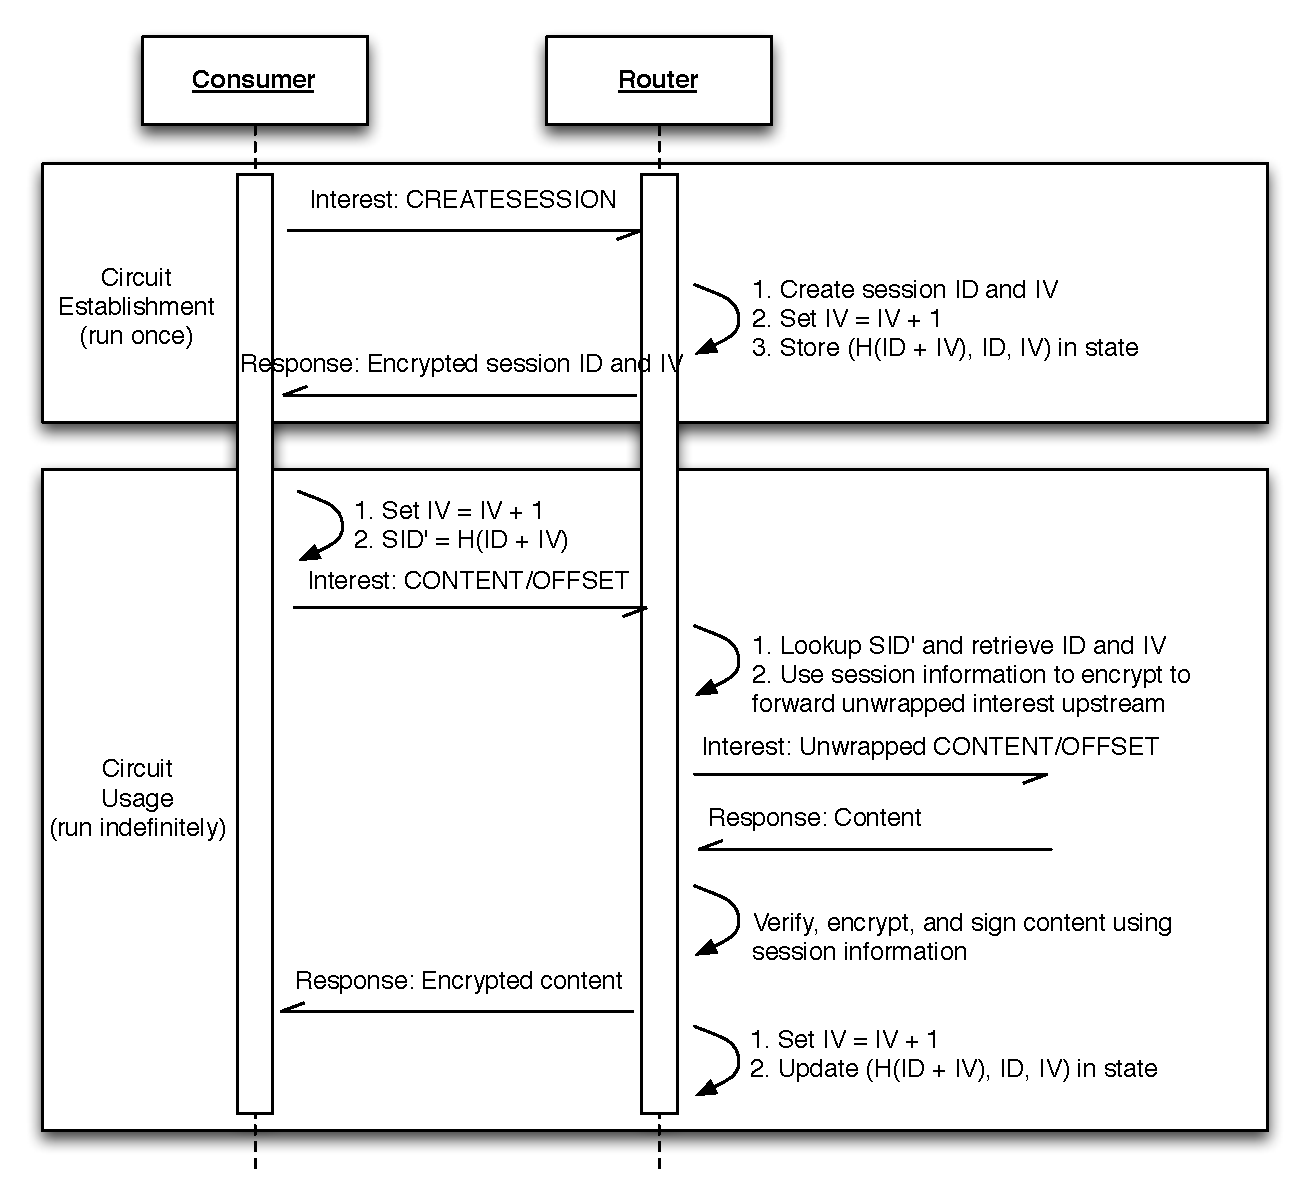
\includegraphics[scale=0.65]{./images/circuit_usage.pdf}
% \end{center}
% \caption{Visual depiction of the interaction between the consumer and the first hop router for the handshake-based variant. The procedure repeats in the same manner for all further upstream routers after each interest is unrolled and resulting content is encrypted.}
% \label{fig:circuit_usage}
% \end{figure*}

\subsection{Online Session Establishment and Circuit Usage} \label{sec:piggyback}
As previously mentioned, sessions may be created via the handshake technique or online. The process for online state initialization is very similar to the handshake routine with the following exceptions:
\begin{itemize}
  \item The \emph{first} interest $\mathsf{int}$:$1$ issued by the consumer is appended with the encrypted state information (minus the session index) similar to as is done in the handshake variant. The session index $\mathsf{SID}$ is still appended to the interest before the state information. This enables the anonymizing proxies to check for the presence of the session index in their state table. If an entry is not found, the remainder of the interest is decrypted and treated as the initial state information.
  \item All \emph{subsequent} interests $\mathsf{int}$:$i$ ($i > 1$) are prepended with the session index and \emph{padded} with an $l$ bits of data so that $|\mathsf{int}$:$1| = |\mathsf{int}$:$i|$ (i.e., the length of all interests are equal). Since the concatenation of the session identifier and the state information is indistinguishable from the concatenation of a different session identifer and random pad, an adversary cannot distinguish between $\mathsf{int}$:$1$ and $\mathsf{int}$:$i$.
\end{itemize}
Beyond these changes, the operation and usage of the circuits remains the same for consumers and anonymizing proxies. We omit algorithmic details about the above differences since they should be clear from context.

\subsection{Interest Flow Control via Windowing} \label{sec:windowing}
To further increase the throughput of {\sf AND}, the design makes use of a flow control mechanism analogous to the sliding window technique used in standard TCP implementations. In particular, {\sf AND} uses a global maximum window size $w$ that refers to the maximum number of interests that can be issued asynchronously without being acknowledged. The behavior of the interest sliding window will then proceed as follows:
\begin{itemize}
  \item All parties, including the consumer and each AR participating in an anonymous circuit, will maintain four pointers, $\mathsf{WindowStart}$, $\mathsf{WindowEnd}$, $\mathsf{KeyStart}$, and $\mathsf{KeyEnd}$, where $\mathsf{WindowEnd} - \mathsf{WindowStart} \leq w$ will always be an invariant. To start, $\mathsf{WindowStart} = \mathsf{WindowEnd} = 0 = \mathsf{KeyStart} = \mathsf{KeyEnd} = 0$.
  \item When an interest is to be issued or forwarded, the party will check to ensure that $\mathsf{WindowEnd} - \mathsf{WindowStart} < w$, and if so interest is sent/forwarded and $\mathsf{WindowEnd}$ is incremented by one. In addition, the keystream at the consumer (for each AR) or AR is pumped by $M$ bits and $\mathsf{KeyEnd}$ is incremented by $M$, where $M$ is the largest piece of content received thus far. Otherwise, the interest is buffered at the consumer or AR. 
  \item When a piece of content arrives that corresponds to some interest issued between $\mathsf{WindowStart}$ and $\mathsf{WindowEnd}$, $\mathsf{WindowStart}$ is incremented by one and an event is triggered forcing the party to check their interest buffers for new intersts to be sent. In addition, $\mathsf{KeyStart}$ is incremented by the size of the content, and checks to see if the maximum content size $M$ needs to be updated.
\end{itemize}
Using this technique, if a router receives an interest for a particular anonymous circuit when $\mathsf{WindowEnd} - \mathsf{WindowStart} \geq w$, then the interest is dropped. Interest and content flow control and correct functionality of the consumer guarantees that interests will not be issued when the window is full. 

Also, while all parties must share the same window size, the consumer $w$ is free to change the window size to adapt to the state of the network. For instance, if there is very little end-to-end latency for content, then the consumer may wish to increase the size of the window. In order to support such dynamic windowing, the consumer must inform all routers in an anonymous circuit of the desired window size. {\sf AND} supports this by appending the window size to the session index $\mathsf{SIndex}_i$ for each $r_i$ in a circuit. In order to ensure that no two interests are distinguishable by this window size $w$, it is also masked by a random one-time pad $p$ (i.e. $w' = w \oplus p$, where $w$ is interpreted as an integer encoded in binary) that is included in the encrypted interest. In other words, once an interest is decrypted the pad $p$ is recovered, and then the router computes $w = w' \oplus p$. If $w$ is larger than the stored value associated with the circuit, then the new result is simply updated and operation proceeds as normal. Otherwise, the router enters a ``backoff'' state where it waits for content to be returned and the resulting window size to return to normal before issuing any further interests. This dynamic windowing method is currently not implemented in the {\sf AND} system.

\begin{figure*}[ht!]
\begin{center}
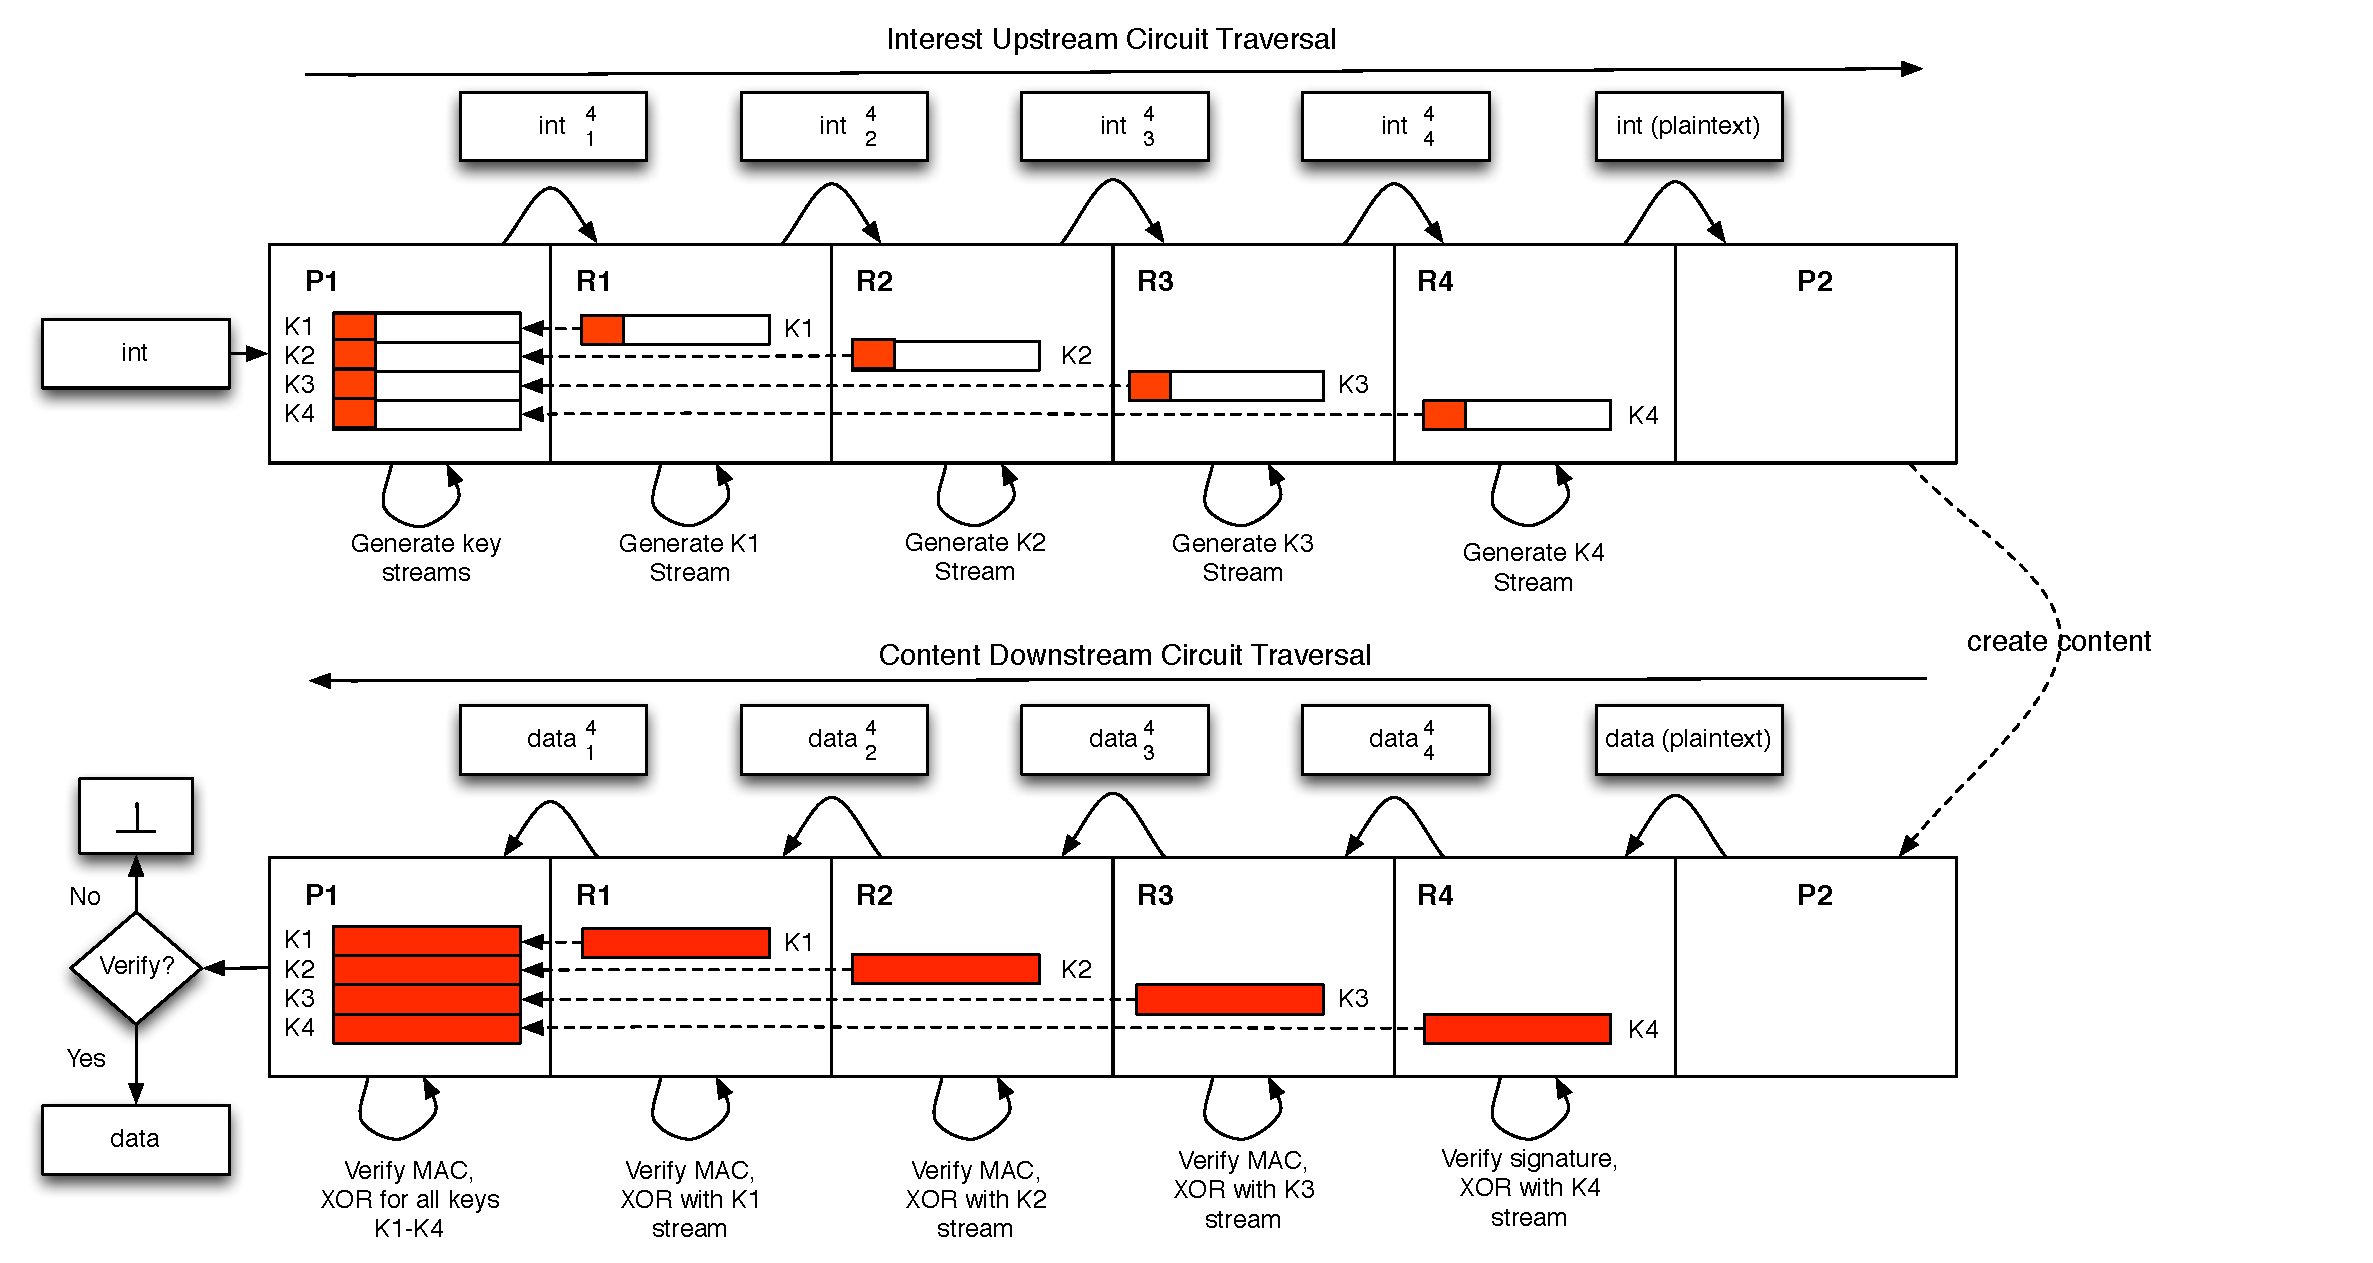
\includegraphics[scale=0.45]{./images/ctr_split.pdf}
\end{center}
\caption{Visual depiction of window-based keystream precomputation during upstream interest traversal.}
\label{fig:circuit}
\end{figure*}

\section{Implementation} \label{sec:introduction}
TODO
\section{Security Analysis} \label{sec:security}
In order to assess the security of {\sf AND} it is important to first define an adversarial model and corresponding definition of security. To this end, we define an adversarial model for {\sf AND} that has the same capabilities as presented in \cite{andana}: Deploy compromised routers, Compromise existing routers, Control content producers, Deploy compromised caches, and Observe and replay traffic. Furthermore, any of these actions or capabiltiies can be carried out adaptively (i.e., in response to status updates from the network or based on the adversary's observations). We also note that the time required to carry out an attack is non-negligibly larger than the average RTT for an interest-content exchange in order to make this model realistic. 

We also emphasize that the fundamental differences between the design of {\sf AND\=aNA} and {\sf AND} are that, in {\sf AND}, each adjacent router will share a private MAC key used for efficient content signature generation (and, optionally, verification) and sessions are identified by the output of $H$ (rather than encrypting and decrypting interests using expensive asymmetric procedures). Accordingly, the proofs of anonymity and privacy need to be augmented to take this into account. The remainder of the design is syntactically equivalent to that of {\sf AND\=aNA}, and so we may restate the theoreoms without proof. However, in doing so, we generalize them to circuits of length $n \geq 2$. 

\begin{thm}
Consumer $u \in (\mathsf{C} \setminus \mathsf{C}_{\mathcal{A}})$ has consumer anonymity in configuration $C$ with respect to adversary $\mathcal{A}$ if there exists $u \not= u'$ such that any of the following conditions hold:
\begin{enumerate}
	\item $u, u' \in \mathsf{AS}_{\mathcal{A}}^{C_4(u)}$
	\item There exists ARs $r_i$ and $r_i'$ such that $r_i,r_i' \notin \mathsf{R}_{\mathcal{A}}$, both $r_i$ and $r_i'$ are on the circuit traversed by $C_4(u) = \overline{\mathsf{int}}_1^n$.
\end{enumerate}
\end{thm}
\begin{proof}
See \cite{andana}.
\end{proof}

\begin{thm}
Consumer $u$ has producer anonymity in configuration $C$ with respect to producer $p \in \mathsf{P}$ and adversary $\mathcal{A}$ if there exists a pair of ARs $r_i$ and $r_i'$ such that $r_i$ and $r_i'$ (for some uncompromised entity $u \notin \mathsf{C}_{\mathcal{A}}$) are on the path traversed by $C_4(u) = \overline{\mathsf{int}}_1^n$, $C_1(u) = C_1(u')$, and $C_3(u) = p \not= C_3(u')$.
\end{thm}
\begin{proof}
See \cite{andana}.
\end{proof}

\begin{cor}
Consumer $u \in (\mathsf{C} \setminus \mathsf{C}_{\mathcal{A}})$ and producer $p \in \mathsf{P}$ are unlinkable in configuration $C$ with respect to adversary $\mathcal{A}$ if $p$ has producer anonymity with respect to $u$'s interests or $u$ has consumer anonymity and there exists a configuration $C' \equiv_{\mathcal{A}} C$ where $C'(u') = C(u)$ with $u' \not= u$ and $u'$'s interests have a destination different from $p$. 
\end{cor}

In addition to security, we must also be concerned about the correct functioning of each AR supporting a session between two parties. In this context, we (informally) define session correctness as the ability of a consumer to correctly decrypt content that is generated \emph{in response to} its original interest. That is, if a consumer issues an interest, it should be able to correctly decrypt the content that it receives. The following factors impact the correctness of the session:
\begin{enumerate}
  \item Each AR $r_1,\dots,r_n$ on the consumer-to-producer circuit should correctly recover the session identifier associated with the current session. 
  \item The session key streams should only be advanced upon the receipt of an interest corresponding to the consumer who initiated the session or content that is generated from the upstream router (potentially the producer) in the circuit.
\end{enumerate}

The first item is necessary in order for each AR to correctly decrypt interests, encrypt content, and perform content signature generation and verification. The second item is necessary so that all content can be correctly decrypted by the consumer. We claim that, given a CCA-secure public key encryption scheme, the probability that either one of these factors being violated by an adversary $\mathcal{A}$ is negligible. Let $\mathsf{ForgeSession}$ and $\mathsf{KeyJump}$ denote the events corresponding to instances where an adversary creates a ciphertext that maps to a valid session identifier for \emph{some} session currently supported by an AR (i.e., the forged session belongs to the routers session table $\mathsf{ST}$), and the event that an adversary causes the key stream for \emph{some} AR in a consumer-to-producer circuit to fall out of sync with the consumer. By the design of {\sf AND}, it should be clear that $\mathsf{KeyJump}$ occurs when $\mathsf{ForgeSession}$ occurs, since the key stream is only advanced upon receipt of an interest, but may also occur when an adversary successfully forges a MAC tag corresponding to the signature of a piece of content from the upstream router (or producer). We denote this latter event as $\mathsf{ContentMacForge}$. With the motivation in place, we now formally analyze the probabilities of these events occuring below. For notational convenience, we assume that each event only occurs as a result of some adversarial action, so we omit this relation in what follows.

\begin{lemma}
For all probabilistic polynomial-time adversaries $\mathcal{A}$, there exists some negligible function $\mathsf{negl}$ such that
\begin{align*}
\Pr[\mathsf{ForgeSession}] \leq \mathsf{negl}(\kappa).
\end{align*}
\end{lemma}
\begin{proof}
By the design of {\sf AND}, we know that session identifiers are computed as the output of a collision resistant hash function $H : \{0,1\}^* \to \{0,1\}^{m}$, where $m = \mathsf{poly}(\kappa)$ (i.e. polynomial in the global security parameter). Consequently, forging a session identifier \emph{without} the input to $H$ implies that a collision was found, thus violating collision resistance of $H$. Thus, forging a session is equally hard as finding a collision in $H$, or more formally, $\Pr[\mathsf{Collision}(H) = 1] = \Pr[\mathsf{ForgeSession}]$. By the properties of collision resistance of $H$ which states that $\Pr[\mathsf{Collision}(H) = 1] \leq \mathsf{negl}(\kappa)$ for some negligible function $\mathsf{negl}$, it follows that $\Pr[\mathsf{ForgeSession}] \leq \mathsf{negl}(\kappa)$. 

% TODO: asusme that some session is forged... session identifiers are created from hashing the session ID as per the above design, so a forgery implies a collision in the hash function. If we assume a CRH hash, then forgery implies contradiction, and we're done.
\end{proof}

\begin{lemma}
For all probabilistic polynomial-time adversaries $\mathcal{A}$, there exists some negligible function $\mathsf{negl}$ such that
\begin{align*}
\Pr[\mathsf{ContentMacForge}] \leq \mathsf{negl}(\kappa).
\end{align*}
\end{lemma}
\begin{proof}
By the design of {\sf AND}, the MAC scheme $\Pi$ used for content symmetric content signature generation and verification is defined as $\Pi = (\mathsf{Gen}, \mathsf{Mac}, \mathsf{Ver})$, where $\mathsf{Gen}$ generates the secret key $k$ used in the scheme, $\mathsf{Mac}_k(m)$ outputs the MAC tag $t := F_k(m)$ for some pseudorandom function $F$, and $\mathsf{Ver}_k(m, t)$ outputs $1$ if $t = \mathsf{Mac}_k(m)$ and $0$ otherwise. This is known and proven to be a secure MAC scheme [does this warrant citation?], meaning that for all probabilistic polynomial-time adversaries $\mathcal{A}$ there exists a negligible function $\mathsf{negl}$ such that $\Pr[\mathsf{MacForce}_{\mathcal{A},\Pi}(1^{\kappa}) = 1] \leq \mathsf{negl}(\kappa)$, and since $\mathsf{ContentMacForce}$ occurs exactly when the even $\mathsf{MacForce}$ occurs, we have that $\Pr[\mathsf{ContentMacForge}] \leq \mathsf{negl}(\kappa)$.

% TODO: assume secure MAC scheme based on PRF is used, a forgery in the MAC scheme therefore relies on the PRFness of SipHash... If this holds, then ContentMacForge is negligible.
\end{proof}

\begin{lemma}
For all probabilistic polynomial-time adversaries $\mathcal{A}$, there exists some negligible function $\mathsf{negl}$ such that
\begin{align*}
\Pr[\mathsf{KeyJump}] \leq \mathsf{negl}(\kappa).
\end{align*}
\end{lemma}
\begin{proof}
By the design of {\sf AND}, it follows that $\Pr[\mathsf{KeyJump}] = \Pr[\mathsf{ForgeSession}] + \Pr[\mathsf{ContentMacForce}]$, and since the sum of two negligible functions is also negligible, it follows that there exists some negligible function $\mathsf{negl}$ such that $\Pr[\mathsf{KeyJump}] \leq \mathsf{negl}(\kappa)$.
\end{proof}

\begin{thm}
Session correctness of {\sf AND} is only violated with negligible probability.
\end{thm}
\begin{proof}
This follows immediately from Lemmas 1, 2, and 3 and the fact that the sum of two negligible functions is also negligible.\footnote{This sum comes from the fact that the probability of the ``failure'' events occurring must be taken into account in both directions of the session.} 
\end{proof}
\section{Performance} \label{sec:performance}
TODO

\section{Conclusion}
TODO

\section{Acknowledgments}
TODO

% The following two commands are all you need in the
% initial runs of your .tex file to
% produce the bibliography for the citations in your paper.
\bibliographystyle{abbrv}
\bibliography{ref}  % sigproc.bib is the name of the Bibliography in this case

% \appendix
% %Appendix A
% \section{Headings in Appendices}
% The rules about hierarchical headings discussed above for
% the body of the article are different in the appendices.
% In the \textbf{appendix} environment, the command
% \textbf{section} is used to
% indicate the start of each Appendix, with alphabetic order
% designation (i.e. the first is A, the second B, etc.) and
% a title (if you include one).  So, if you need
% hierarchical structure
% \textit{within} an Appendix, start with \textbf{subsection} as the
% highest level. Here is an outline of the body of this
% document in Appendix-appropriate form:
% \subsection{Introduction}
% \subsection{The Body of the Paper}
% \subsubsection{Type Changes and  Special Characters}
% \subsubsection{Math Equations}
% \paragraph{Inline (In-text) Equations}
% \paragraph{Display Equations}
% \subsubsection{Citations}
% \subsubsection{Tables}
% \subsubsection{Figures}
% \subsubsection{Theorem-like Constructs}
% \subsubsection*{A Caveat for the \TeX\ Expert}
% \subsection{Conclusions}
% \subsection{Acknowledgments}
% \subsection{Additional Authors}
% This section is inserted by \LaTeX; you do not insert it.
% You just add the names and information in the
% \texttt{{\char'134}additionalauthors} command at the start
% of the document.
% \subsection{References}
% Generated by bibtex from your ~.bib file.  Run latex,
% then bibtex, then latex twice (to resolve references)
% to create the ~.bbl file.  Insert that ~.bbl file into
% the .tex source file and comment out
% the command \texttt{{\char'134}thebibliography}.
% % This next section command marks the start of
% % Appendix B, and does not continue the present hierarchy
% \section{More Help for the Hardy}
% The acm\_proc\_article-sp document class file itself is chock-full of succinct
% and helpful comments.  If you consider yourself a moderately
% experienced to expert user of \LaTeX, you may find reading
% it useful but please remember not to change it.
% \balancecolumns
% % That's all folks!

\end{document}
